\documentclass[12pt]{article}
\lineskip=0pt % https://tex.stackexchange.com/a/349882

\usepackage[skins, breakable, raster]{tcolorbox}
\tcbsetforeverylayer{
  skin=enhanced jigsaw,
  fonttitle=\large,
  colback=white,
  subtitle style={colback=gray, fontupper=\normalsize\bfseries},
  left=-0.25pt, right=-0.25pt, top=0pt, bottom=0pt,
  nobeforeafter,
  boxrule=0.5pt,
  % multicol compatibility
  breakable, height fixed for=first,
  pad at break*=0pt, pad before break*=0pt, pad after break=0pt,
  break at=-\baselineskip/0pt
}

\usepackage{multicol}
\usepackage{geometry}
\geometry{
	paperheight=420mm, paperwidth=594mm,
	tmargin=5pt, bmargin=5pt, hmargin=5pt,
	noheadfoot=true
}

\usepackage{graphicx}
\graphicspath{{./images/}}

\usepackage{xcolor}
\usepackage{soul}
\definecolor{lightgray}{gray}{0.87}
\newcommand{\hlfancy}[2]{\sethlcolor{#1}\hl{#2}}
\newcommand{\hlfancymath}[2]{%
    \begingroup
    \mathchoice
        {\colorbox{#1}{$\displaystyle #2$}}%
        {\colorbox{#1}{$\textstyle #2$}}%
        {\colorbox{#1}{$\scriptstyle #2$}}%
        {\colorbox{#1}{$\scriptscriptstyle #2$}}%
    \endgroup
}
\newcommand{\hlfancytall}[2]{%
    \begingroup
    \setlength{\fboxsep}{0pt}%
    \colorbox{#1}{#2}%
    \endgroup
}
\usepackage{parskip}
\setlength{\parskip}{0pt}
\usepackage[fleqn]{amsmath}
\setlength{\mathindent}{0pt}
\setlength{\parindent}{0pt}
\usepackage[inline]{enumitem}
% ref: https://tex.stackexchange.com/a/660129
\setlist{leftmargin=*, labelsep=1pt, itemsep=1pt}
\setlist[itemize]{label=$\bullet$}
\usepackage{amssymb, mathabx, esdiff}
\usepackage{tabularray}
\newcommand{\dd}[1]{\,d#1} % for differentials in integrals
\DeclareMathOperator{\var}{Var}
\DeclareMathOperator{\cov}{cov}
\DeclareMathOperator{\N}{N}
\DeclareMathOperator{\tdist}{t}

% fixes spacing
% ref: https://tex.stackexchange.com/a/2610
\let\originalleft\left
\let\originalright\right
\renewcommand{\left}{\mathopen{}\mathclose\bgroup\originalleft}
\renewcommand{\right}{\aftergroup\egroup\originalright}

\pagestyle{empty}

\begin{document}
% https://tex.stackexchange.com/a/237763
% for align environment spacing
\setlength{\abovedisplayskip}{0pt}
\setlength{\belowdisplayskip}{0pt}
\setlength{\abovedisplayshortskip}{0pt}
\setlength{\belowdisplayshortskip}{0pt}
\setlength{\jot}{1pt}

\setlength\columnsep{0pt}

\begin{multicols*}{5}
	\begin{tcolorbox}[title=Probability]
		\begin{tblr}{
				cells={mode=dmath},
				colspec={c|c},
				leftsep=0pt, rightsep=0pt,
				column{1}={rightsep=5pt},
				column{2}={leftsep=5pt},
			}
			{^nP_k}= \dfrac{n!}{(n-k)!} = {^nC_k} \times k!
			 &
			{^nC_k} = \dfrac{n!}{k!(n-k)!} = {^nP_k}\ /\ k!

		\end{tblr}
		\vspace*{1pt}\hrule\vspace*{1pt}

		\begin{align*}
			P(A) & = P(A \cap B) + P(A \cap B')          \\
			     & = P(B)P(A \mid B) + P(B')P(A \mid B')
		\end{align*}

		\begin{align*}
			P(B \mid A) & = \dfrac{P(A \cap B)}{P(A)} \ = \dfrac{P(B)P(A \mid B)}{P(A)} \\
			            & = \dfrac{P(A \cap B)}{P(B)P(A \mid B) + P(B')P(A \mid B')}
		\end{align*}

		\vspace{\baselineskip}
		Bayes Theorem: $P(B_k  \mid  A) = \dfrac{P(B_k)P(A \mid B_k)}{\displaystyle\sum{P(B_i)P(A \mid B_i)}}$ \\
		\begin{tblr}{
				colspec={l|l},
				leftsep=0pt, rightsep=0pt,
				column{1}={rightsep=5pt},
				column{2}={leftsep=5pt},
			}
			Prior: $P(B_k)$
			 & Posterior: $P(B_k \mid A)$
			\\
			Likelihood: $P(A \mid B_k)$
			 & Evidence: $P(A)=\displaystyle\sum P(B_i)P(A \mid B_i)$
		\end{tblr}

		\vspace*{1pt}\hrule\vspace*{1pt}

		\begin{tblr}{
				cells={mode=dmath},
				colspec={c|c},
				leftsep=0pt, rightsep=0pt,
				column{1}={rightsep=5pt},
				column{2}={leftsep=5pt},
			}
			\begin{aligned}[t]
				 & \text{Independent:}                       \\
				 & P(A \cap B) = P(A)P(B)                    \\
				 & \Leftrightarrow P(B \mid A) = P(B)        \\
				 & \Leftrightarrow P(A \mid B) = P(A)        \\
				 & \Rightarrow \text{not mutually exclusive}
			\end{aligned}
			 &
			\begin{aligned}[t]
				 & \text{Mutually exclusive:}                \\
				 & A \cap B = \emptyset                      \\
				 & \Leftrightarrow P(A \cup B) = P(A) + P(B) \\
				 & \Rightarrow \text{not independent}
			\end{aligned}
		\end{tblr}
	\end{tcolorbox}

	\newcolumn

	\begin{tcolorbox}[title=Data]
		Discrete: \\
		PMF: $f(x) = P(X = x)$ \\
		CDF: $F(x) = P(X \leq x) = \displaystyle\sum_{u \leq x}{f(u)}$

		\begin{align*}
			1 - F(x) & = 1 - P(X \leq x) \\
			         & = P( X > x)
		\end{align*}

		\begin{align*}
			F(b) - F(a) & = P(X \leq b) - P(X \leq a) \\
			            & = P(a < X \leq b)
		\end{align*}

		\begin{align*}
			f(x) & = P(X = x) = P(X \leq x) - P(X < x) \\
			     & = F(x) - F(x-)
		\end{align*}

		\vspace{\baselineskip}
		Continuous: \\
		PDF: $\displaystyle\int_a^b f(x)\dd{x} = P(a \leq X \leq b)$ \\
		CDF: $F(x) = P(X \leq x) =  \displaystyle\int_{-\infty}^{x}f(t)\dd{t}$

		\begin{align*}
			1 - F(x) & = 1 - P(X \leq x) \\
			         & = P( X \geq x)
		\end{align*}

		\begin{align*}
			F'(x) & = \diff{}{x}\displaystyle\int_{-\infty}^{x}f(t)\dd{t} \\
			      & = f(x)
		\end{align*}

		\vspace{\baselineskip}
		Joint Discrete: \\
		PMF: $f_{X, Y}(x, y) = P(X = x,\ Y = y) = P(X = x \cap Y = y)$ \\
		CDF: $F_{X, Y}(x, y) = P(X \leq x,\ Y \leq y) = \displaystyle\sum_{u \leq x}\sum_{v \leq y} f_{X, Y}(u, v)$ \\
		Marginal: $f_X(x) = P(X=x) = \displaystyle\sum_y f_{X, Y}(x, y)$

		\vspace{\baselineskip}
		Joint Continuous: \\
		PDF: $\displaystyle\int\int_D f_{X, Y}(x, y)\dd{x}\dd{y} = P((x, y) \in D)$ \\
		Marginal: $f_X(x) = \displaystyle\int_{-\infty}^{\infty}f_{X, Y}(x, y)\dd{y}$

		\vspace{\baselineskip}
		Conditional: $f_{Y \mid X}(y \mid x) = \dfrac{f_{X, Y}(x, y)}{f_X(x)}$

		\vspace{\baselineskip}
		Independent random variables:
		\begin{align*}
			 & \Leftrightarrow f_{X,Y}(x,y)=f_X(x)f_Y(y)   \\
			 & \Leftrightarrow F_{X,Y}(x,y)=F_X(x)F_Y(y)   \\
			 & \Leftrightarrow f_{Y\mid X}(y\mid x)=f_Y(y) \\
			 & \Leftrightarrow f_{X\mid Y}(x\mid y)=f_X(x)
		\end{align*}

		\vspace{\baselineskip}
		Independence shortcut: \\
		Support $R_{X,Y}=R_X\times R_Y$ and
		$f_{X,Y}(x,y)=C \cdot g_1(x)g_2(y)$ over the support.

		\vspace{\baselineskip}
		Marginals from factorisation: \\
		$f_X(x)=C \cdot g_1(x)\displaystyle\sum_{y}g_2(y)$ or $ =C \cdot g_1(x)\displaystyle\int_{y}g_2(y)\,dy$\\
		$f_Y(y)=C \cdot g_2(y)\displaystyle\sum_{x}g_1(x)$ or $=C \cdot g_2(y)\displaystyle\int_{x}g_1(x)\,dx$

		\vspace{\baselineskip}
		$n$-th percentile $p_n$: $\text{CDF}(p_n) = n/100$

		\vspace{\baselineskip}
		$\mu_X = E(X) = \displaystyle\sum_{x}xf(x) \text{ or} =\displaystyle\int_{x}xf(x)\dd{x}$ \\
		$E(g(X)) = \displaystyle\sum_{x}g(x)f(x) \text{ or} =\displaystyle\int_{x}g(x)f(x)\dd{x}$ \\
		$E(aX + b) = aE(X) + b$ \\
		$E(X + Y) = E(X) + E(Y)$ \\
		$E\left(\displaystyle\sum X_i\right) = \displaystyle\sum E(X_i)$

		\begin{align*}
		{\sigma_X}^2 = \var(X) & = E[(X - \mu_X)^2]                                                                                \\
		                                      & = \displaystyle\sum_{x}(x - \mu_X)^2f(x) \text{ or} =\displaystyle\int_{x}(x - \mu_X)^2f(x)\dd{x} \\
		                                      & = E[X^2] - E[X]^2
		\end{align*}
		$\var(aX + b) = a^2\var(X)$ \\
		$\var(X \pm Y) = \var(X) + \var(Y) \pm 2\cov(X, Y)$ \\
		$\var\left(\displaystyle\sum X_i\right) = \displaystyle\sum \var(X_i) + 2\displaystyle\sum_{m>n} \cov(X_m, X_n)$

		\begin{align*}
			\cov(X,Y) & = E[(X - \mu_X)(Y - \mu_Y)]                                                                 \\
			          & = \displaystyle\sum_{y}\displaystyle\sum_{x}(x - \mu_X)(y - \mu_Y)f_{X,Y}(x, y)             \\
			\text{or} & = \displaystyle\int_{y}\displaystyle\int_{x}(x - \mu_X)(y - \mu_Y)f_{X,Y}(x, y)\dd{x}\dd{y} \\
			          & = E[XY] - E[X]E[Y]
		\end{align*}
		$\cov(aX+c_1, bY+c_2) = ab\cov(X, Y)$ \\
		$\cov(X,Y) = \cov(Y,X)$ \\
		$\cov(X + Y, Z) = \cov(X, Z) + \cov(Y, Z)$
		\begin{align*}
			X \perp Y & \Rightarrow \cov(X,Y)=0                  \\
			          & \Rightarrow \var(X\pm Y)=\var(X)+\var(Y)
		\end{align*}

		\vspace{\baselineskip}
		$\rho(X, Y) = \dfrac{\cov(X, Y)}{\sigma_X\sigma_Y}$

		\vspace{\baselineskip}
		Zipf's law for the $x$-th most popular item: \\
		PMF: $f(x) = \dfrac{c}{x},\ x\in\{1\ ..\ n\}$

		\vspace{\baselineskip}
		Benford's law for leading digits: \\
		PMF: $f(d) = \log_{10}\left(1 + \dfrac{1}{d}\right),\ d\in\{1\ ..\ 9\}$
	\end{tcolorbox}

	\newcolumn

	\begin{tcolorbox}[title=Data]
		$\overline{X} = \dfrac{1}{n}\displaystyle\sum X_i$

		\vspace{\baselineskip}
		$\mu_{\overline{X}} = E(\overline{X}) = E(X) = \mu$ \\
		$\sigma_{\overline{X}}^2 = \var(\overline{X}) = \dfrac{\var(X)}{n} = \sigma^2/n$ \\
		LLN: $n \to \infty \Rightarrow \overline{X} \xrightarrow{p} \mu$ \\
		CLT: $n \to \infty \Rightarrow \dfrac{\overline{X} - \mu}{\sqrt{\sigma^2/n}} \xrightarrow{d} \N(0, 1)$
		for i.i.d with finite mean and variance

		\begin{align*}
			S^2 & = \dfrac{1}{n-1}\displaystyle\sum^n (X_i - \overline{X})^2                                          \\
			    & = \dfrac{1}{n-1}\displaystyle\sum^n X_i^2 - \dfrac{n}{n-1}\overline{X}^2                            \\
			    & = \dfrac{1}{n-1}\displaystyle\sum^n X_i^2 - \dfrac{1}{n(n-1)}\left(\displaystyle\sum^n X_i\right)^2
		\end{align*}

		\vspace{\baselineskip}
		Given i.i.d. $X_i \sim \N(0, 1)$, \hlfancytall{lightgray}{$U = \displaystyle\sum^n X_i^2 \sim \chi^2(n)$} \\
		$E(U) = n$ \\
		$\var(U) = 2n$ \\
		For large $n$, $\chi^2(n) \approx \N(n, 2n)$ \\
		\noindent
		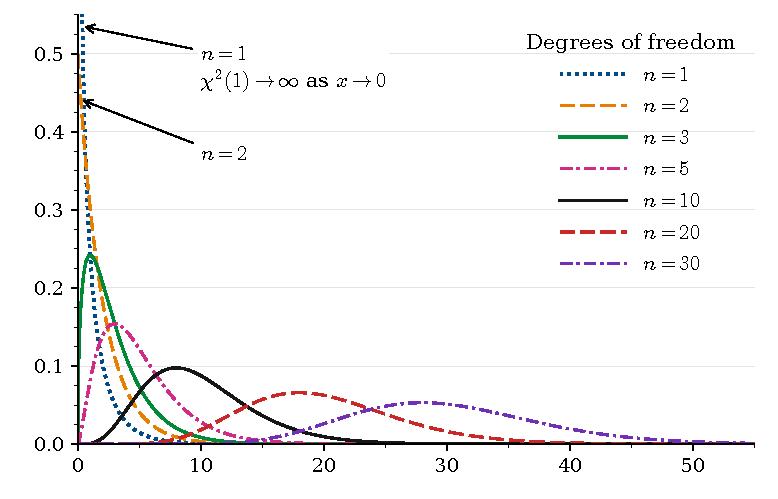
\includegraphics[width=\linewidth]{chi_squares.pdf}

		Given independent $\chi^2(m)$, $\chi^2(n)$, $\chi^2(m) + \chi^2(n) \sim \chi^2(m + n)$ \\
		$\dfrac{X_i - \mu}{\sigma} \sim \N(0, 1) \Rightarrow \displaystyle\sum^n\left(\dfrac{X_i - \mu}{\sigma}\right)^2 = \dfrac{\sum (X_i - \mu)^2}{\sigma^2} \sim \chi^2(n)$
		\begin{align*}
			\hlfancymath{lightgray}{\dfrac{S^2(n-1)}{\sigma^2}}
			 & = \dfrac{\sum (X_i - \overline{X})^2(n-1)}{(n-1)\sigma^2} \\
			 & = \dfrac{\sum (X_i - \overline{X})^2}{\sigma^2}           \\
			 & \hlfancymath{lightgray}{\sim \chi^2(n - 1)}
		\end{align*}
		for i.i.d. normal sample

		\begin{align*}
			P(S^2 \geq c) & = P\left(\dfrac{S^2(n-1)}{\sigma^2} \geq \dfrac{c(n-1)}{\sigma^2}\right) \\
			           & = P\left(\chi^2(n-1) \geq \dfrac{c(n-1)}{\sigma^2}\right)
		\end{align*}
		Assuming $\sigma = \sigma_0$, \hlfancytall{lightgray}{test statistic $= \dfrac{s^2(n-1)}{\sigma^2_0}$} \\
		Compare with \hlfancytall{lightgray}{$\chi^2(n-1)$} critical value table to reject assumption.

		\vspace{\baselineskip}
		Given independent $Z \sim \N(0, 1)$ and $U \sim \chi^2(n)$, \\
		\hlfancytall{lightgray}{$T = \dfrac{Z}{\sqrt{U/n}} \sim \tdist(n)$} \\
		$E(T) = 0$ \\
		$\var(T) = \dfrac{n}{n-2}$ \\
		For large $n$, $\tdist(n) \approx \N(0, 1)$ \\
		\noindent
		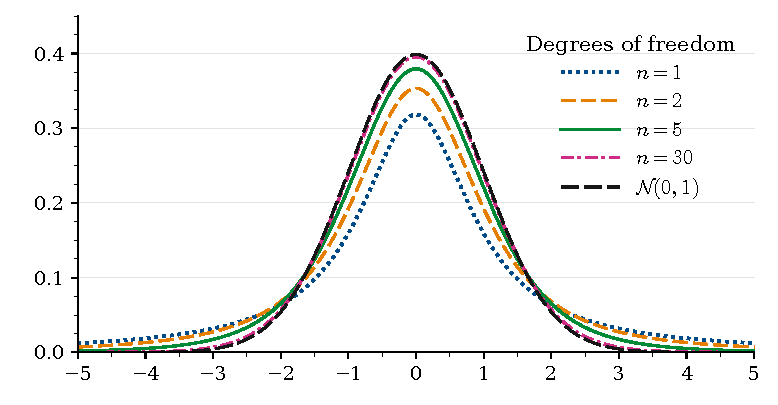
\includegraphics[width=\linewidth]{t_distributions.pdf}

		\begin{align*}
			\hlfancymath{lightgray}{\dfrac{\overline{X} - \mu}{\sqrt{S^2/n}}}
			 & = \dfrac{\overline{X} - \mu}{\sqrt{\dfrac{S^2(n-1)\sigma^2}{\sigma^2(n-1)n}}}                  \\
			 & = \dfrac{\overline{X} - \mu}{\sqrt{\dfrac{\sigma^2}{n}}\sqrt{\dfrac{S^2(n-1)}{\sigma^2(n-1)}}} \\
			 & = \dfrac{\dfrac{\overline{X} - \mu}{\sqrt{\sigma^2/n}}}%
			     {\sqrt{\dfrac{S^2(n-1)}{\sigma^2}\Big/(n-1)}}                            \\
			 & \hlfancymath{lightgray}{\sim \tdist(n - 1)}
		\end{align*}
		for i.i.d. normal sample

		\vspace{\baselineskip}
		Given independent $U \sim \chi^2(m)$, $V \sim \chi^2(n)$, \\
		\hlfancytall{lightgray}{$F = \dfrac{U/m}{V/n} \sim F(m, n)$} \\
		$E(F) = \dfrac{n}{n-2}$ \\
		$\var(F) = \dfrac{2n^2(m+n-2)}{m(n-2)^2(n-4)}$ \\
		Given $F_1 \sim F(m, n)$, $F_2 = \dfrac{1}{F_1} \sim F(n, m)$

		\begin{align*}
			 & P(F_1 \geq F(m, n; \alpha)) = \alpha                                                     \\
			 & \Rightarrow P(\frac{1}{F_1} \leq \frac{1}{F(m, n; \alpha)}) = \alpha                     \\
			 & \Rightarrow P(F_2 \leq \frac{1}{F(m, n; \alpha)}) = \alpha                               \\
			 & \Rightarrow 1 - P(F_2 \geq \frac{1}{F(m, n; \alpha)}) = \alpha                           \\
			 & \Rightarrow P(F_2 \geq \frac{1}{F(m, n; \alpha)}) = 1 - \alpha                           \\
			 & \Rightarrow\!\hlfancymath{lightgray}{F(n, m; 1 - \alpha) = \frac{1}{F(m, n; \alpha)}}
		\end{align*}

		$m \to \infty,\ n\to \infty \Rightarrow F(m,n) \to 1$ \\
		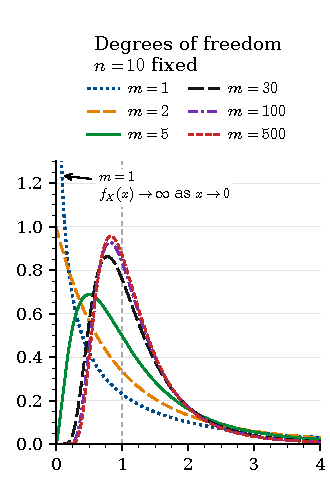
\includegraphics[width=.49\linewidth]{f_varying_m.pdf}
		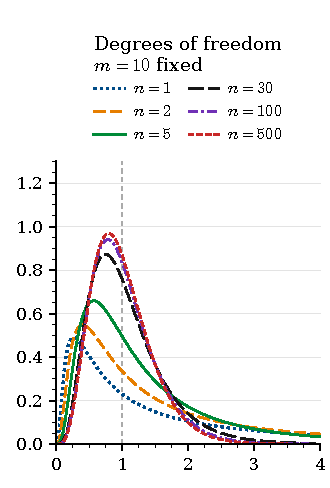
\includegraphics[width=.49\linewidth]{f_varying_n.pdf}

		\begin{align*}
			\hlfancymath{lightgray}{\dfrac{S_1^2/\sigma_1^2}{S_2^2/\sigma_2^2}}
			 & = \dfrac{\dfrac{S_1^2(n_1-1)}{\sigma_1^2}/(n_1-1)}%
			     {\dfrac{S_2^2(n_2-1)}{\sigma_2^2}/(n_2-1)} \\
			 & \hlfancymath{lightgray}{\sim F(n_1 - 1, n_2 - 1)}
		\end{align*}

		Assuming equal variances $\sigma_1 = \sigma_2$, \hlfancytall{lightgray}{test statistic $= \dfrac{s^2_1}{s_2^2}$} \\
		Compare with \hlfancy{lightgray}{$F(n_1 - 1, n_2 - 1)$} critical value table to reject assumption.
	\end{tcolorbox}

	\newcolumn

	\begin{tcolorbox}[title=Data]
		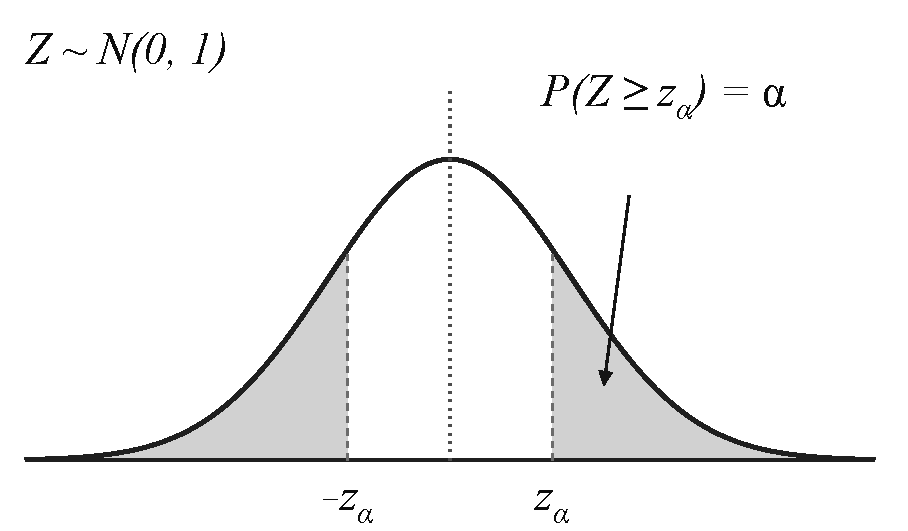
\includegraphics[width=\linewidth]{normal-upper-tail.pdf} \\
		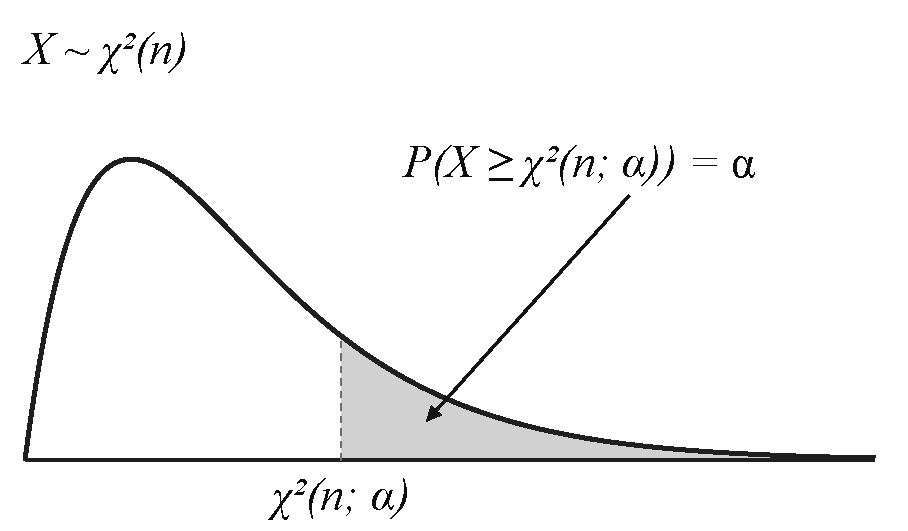
\includegraphics[width=\linewidth]{chi-square-upper-tail.pdf}\\
		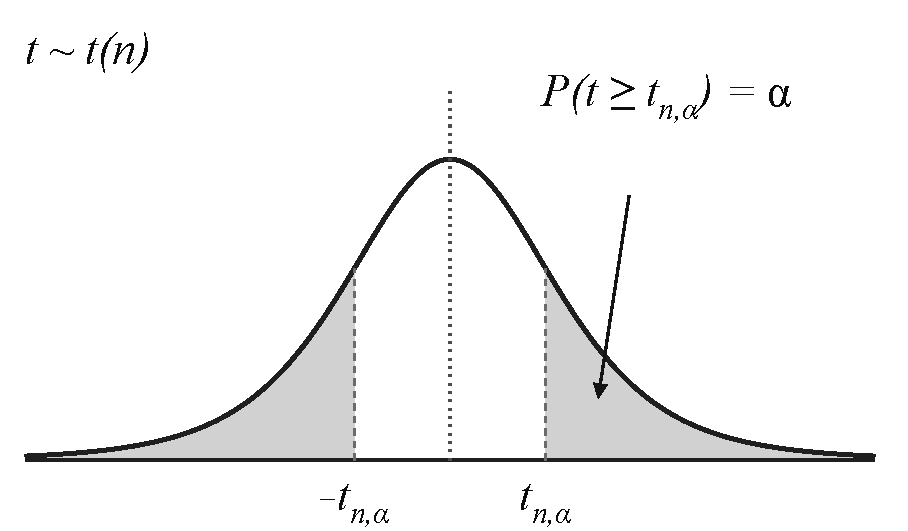
\includegraphics[width=\linewidth]{t-upper-tail.pdf}\\
		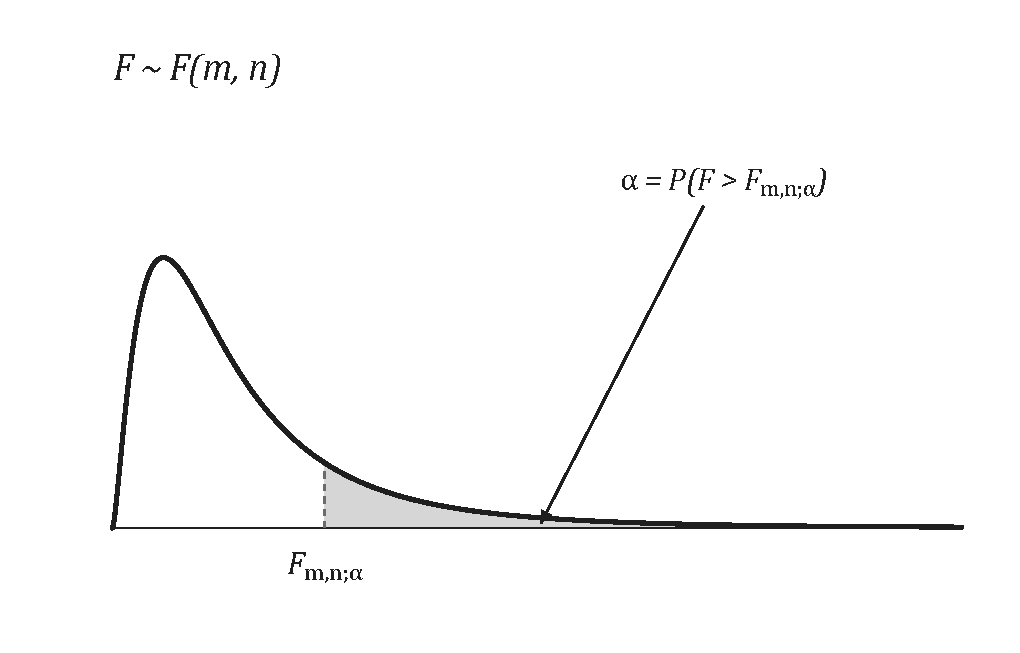
\includegraphics[width=\linewidth]{f-upper-tail.pdf}

		Before computing, the \hlfancy{lightgray}{CI procedure has probability $(1-\alpha)$ of capturing $\mu$.}
		However, after a CI is computed, $\mu$ either lies in it or it does not.
		Thus, we call it a \hlfancy{lightgray}{$100*(1-\alpha)\%$ CI}, and we are \hlfancy{lightgray}{$100*(1-\alpha)\%$ confident} a computed CI contains $\mu$,
		\hlfancy{lightgray}{not that there is probability $(1-\alpha)$} a computed CI contains $\mu$.

		General form for test statistic: $\dfrac{\text{sample val} - \text{population val}}{SE}$ \\
		General form for CI: $\text{sample val} \pm \text{critical value}\times\text{SE}$

		Single sample, \hlfancy{lightgray}{$H_0:\mu=\mu_0$}: \\
		\begin{tblr}{
				colspec={|c|c|c|c|c|c|c|},
				hlines,
				rows={valign=m},
			}
			Population & $\sigma$; $n$
			           & SE
			           & \shortstack{Test statistic\\under $H_0$}
			           & $(1-\alpha)$ CI for $\mu$                             & \shortstack{Maximum error\\of estimate $E$}
			           & \shortstack{Min $n$ for given\\$E$ and $\alpha$}                                                        \\

			Normal     & \shortstack{Known;\\Any}
			           & $\dfrac{\sigma}{\sqrt{n}}$
			           & $Z=\dfrac{\overline X-\mu_0}{\sigma/\sqrt n}$
			           & $\overline x\pm z_{\alpha/2}\dfrac{\sigma}{\sqrt n}$
			           & $E = z_{\alpha/2}\dfrac{\sigma}{\sqrt n}$
			           & $\displaystyle\left\lceil
				             \left(\dfrac{z_{\alpha/2}\cdot \sigma}{E_0}\right)^2
				             \right\rceil$                                                \\

			Any        & \shortstack{Known;\\Large}
			           & $\dfrac{\sigma}{\sqrt{n}}$
			           & $Z\approx\dfrac{\overline X-\mu_0}{\sigma/\sqrt n}$
			           & $\overline x\pm z_{\alpha/2}\dfrac{\sigma}{\sqrt n}$
			           & $E = z_{\alpha/2}\dfrac{\sigma}{\sqrt n}$
			           & $\displaystyle\left\lceil
				             \left(\dfrac{z_{\alpha/2}\cdot \sigma}{E_0}\right)^2
				             \right\rceil$                                                \\

			Normal     & \shortstack{Unknown;\\Small}
			           & $\dfrac{S}{\sqrt{n}}$
			           & $T=\dfrac{\overline X-\mu_0}{S/\sqrt n}$
			           & $\overline x\pm t_{n-1;\alpha/2}\dfrac{s}{\sqrt n}$
			           & $E = t_{n-1;\alpha/2}\dfrac{s}{\sqrt n}$
			           & $\displaystyle\left\lceil
				             \left(\dfrac{t_{n-1;\alpha/2}\cdot s}{E_0}\right)^2
				             \right\rceil$                                                 \\

			Any        & \shortstack{Unknown;\\Large}
			           & $\dfrac{S}{\sqrt{n}}$
			           & $Z\approx\dfrac{\overline X-\mu_0}{S/\sqrt n}$
			           & $\overline x\pm z_{\alpha/2}\dfrac{s}{\sqrt n}$
			           & $E = z_{\alpha/2}\dfrac{s}{\sqrt n}$
			           & $\displaystyle\left\lceil
				             \left(\dfrac{z_{\alpha/2}\cdot s}{E_0}\right)^2
				             \right\rceil$
		\end{tblr}

		Independent two-sample, \hlfancy{lightgray}{$H_0:\mu_1-\mu_2=\delta_0$}: \\
		\begin{tblr}{
				colspec={|c|c|c|c|c|},
				hlines,
				rows={valign=m},
			}
			Variances
			 & Conditions
			 & SE
			 & Test statistic under $H_0$
			 & $(1-\alpha)$ CI for $\mu_1-\mu_2$                                  \\

			\shortstack{Known,\\unequal}
			 & \shortstack{Any;\\$n_1,n_2\ge 30$}
			 & $\sqrt{\dfrac{\sigma_1^2}{n_1}+\dfrac{\sigma_2^2}{n_2}}$
			 & $\displaystyle
				   Z=\frac{(\overline{X}_1-\overline{X}_2)-\delta_0}
				   {\sqrt{\frac{\sigma_1^2}{n_1}+\frac{\sigma_2^2}{n_2}}}$
			 & $\displaystyle
				   (\overline{x}_1-\overline{x}_2)\pm
				   z_{\alpha/2}\sqrt{\frac{\sigma_1^2}{n_1}+\frac{\sigma_2^2}{n_2}}$ \\

			\shortstack{Known,\\unequal}
			 & \shortstack{Normal;\\any $n_1,n_2$}
			 & $\sqrt{\dfrac{\sigma_1^2}{n_1}+\dfrac{\sigma_2^2}{n_2}}$
			 & $\displaystyle
				   Z=\frac{(\overline{X}_1-\overline{X}_2)-\delta_0}
				   {\sqrt{\frac{\sigma_1^2}{n_1}+\frac{\sigma_2^2}{n_2}}}$
			 & $\displaystyle
				   (\overline{x}_1-\overline{x}_2)\pm
				   z_{\alpha/2}\sqrt{\frac{\sigma_1^2}{n_1}+\frac{\sigma_2^2}{n_2}}$ \\

			\shortstack{Unknown,\\unequal}
			 & \shortstack{Any;\\$n_1,n_2\ge 30$}
			 & $\sqrt{\dfrac{S_1^2}{n_1}+\dfrac{S_2^2}{n_2}}$
			 & $\displaystyle
				   Z\approx\frac{(\overline{X}_1-\overline{X}_2)-\delta_0}
				   {\sqrt{\frac{S_1^2}{n_1}+\frac{S_2^2}{n_2}}}$
			 & $\displaystyle
				   (\overline{x}_1-\overline{x}_2)\pm
				   z_{\alpha/2}\sqrt{\frac{s_1^2}{n_1}+\frac{s_2^2}{n_2}}$           \\

			\shortstack{Unknown,\\equal}
			 & \shortstack{Normal;\\$n_1,n_2<30$}
			 & ${S_p\sqrt{\dfrac{1}{n_1}+\dfrac{1}{n_2}}}$
			 & $\displaystyle
				   T=\frac{(\overline{X}_1-\overline{X}_2)-\delta_0}
				   {S_p\sqrt{\frac{1}{n_1}+\frac{1}{n_2}}}$
			 & $\displaystyle
				   (\overline{x}_1-\overline{x}_2)\pm
				   t_{n_1+n_2-2;\alpha/2}\,
				   s_p\sqrt{\frac{1}{n_1}+\frac{1}{n_2}}$                            \\

			\shortstack{Unknown,\\equal}
			 & \shortstack{Any;\\$n_1,n_2\ge 30$}
			 & ${S_p\sqrt{\dfrac{1}{n_1}+\dfrac{1}{n_2}}}$
			 & $\displaystyle
				   Z\approx\frac{(\overline{X}_1-\overline{X}_2)-\delta_0}
				   {S_p\sqrt{\frac{1}{n_1}+\frac{1}{n_2}}}$
			 & $\displaystyle
				   (\overline{x}_1-\overline{x}_2)\pm
				   z_{\alpha/2}\,s_p\sqrt{\frac{1}{n_1}+\frac{1}{n_2}}$
		\end{tblr}

		where \hlfancytall{lightgray}{$s_p^2= \dfrac{s_1^2(n_1-1)+s_2^2(n_2-1)}{n_1+n_2-2}$} is a pooled estimate of the variance

		Dependent two-sample: single sample of paired differences \hlfancy{lightgray}{$D_i = X_i - Y_i$}, \hlfancy{lightgray}{$H_0: \mu_D = \delta_0$} \\
		\begin{tblr}{
				colspec={|c|c|c|},
				hlines,
				rows={valign=m},
			}
			Conditions
			 & \shortstack{Test statistic\\under $H_0$}
			 & $(1-\alpha)$ CI for $\mu_D$                          \\

			\shortstack{Small sample;\\ normal}
			 & $\displaystyle
				   T=\frac{\overline D-\delta_0}{S_D/\sqrt n}$
			 & $\displaystyle
				   \overline d\pm t_{n-1;\alpha/2}\frac{s_D}{\sqrt n}$ \\

			Large sample
			 & $\displaystyle
				   Z\approx\frac{\overline D-\delta_0}{S_D/\sqrt n}$
			 & $\displaystyle
				   \overline d\pm z_{\alpha/2}\frac{s_D}{\sqrt n}$
		\end{tblr}
		\begin{align*}
			\hlfancymath{lightgray}{\overline{D}} & = \dfrac{\sum(X_i - Y_i)}{n}                              \\
			                                      & = \dfrac{\sum X_i}{n} - \dfrac{\sum Y_i}{n}               \\
			                                      & \hlfancymath{lightgray}{ = \overline{X} - \overline{Y{}}}
		\end{align*}

		Hypothesis testing: \\
		\begin{tblr}{
				colspec={|c|c|c|c|},
				hlines,
				rows={valign=m},
			}
			Test
			 & Hypotheses
			 & \shortstack{Reject $H_0$ if}
			 & \shortstack{$p$-value (area under graph)}                                         \\

			Two-sided
			 & \shortstack{$H_0:\theta=\theta_0$\\$H_1:\theta\ne\theta_0$}
			 & $\displaystyle |q_{\mathrm{obs}}|>q_{\alpha/2}$
			 & $\displaystyle
				   2{*}P(Q\ge |q_{\mathrm{obs}}|\mid \theta = \theta_0)$         \\

			Left-tailed
			 & \shortstack{$H_0:\theta\ge\theta_0$\\$H_1:\theta<\theta_0$}
			 & $\displaystyle q_{\mathrm{obs}}<-q_\alpha$
			 & $\displaystyle P(Q\le q_{\mathrm{obs}}\mid \theta = \theta_0)$ \\

			Right-tailed
			 & \shortstack{$H_0:\theta\le\theta_0$\\$H_1:\theta>\theta_0$}
			 & $\displaystyle q_{\mathrm{obs}}>q_\alpha$
			 & $\displaystyle P(Q\ge q_{\mathrm{obs}}\mid \theta = \theta_0)$
		\end{tblr}
		$\theta$ is the population parameter \\
		$q_\mathrm{obs}$ is the calculated test statistic \hlfancy{lightgray}{under $H_0$} \\
		$q_\alpha$ is the upper-tail critical value at significance $\alpha$ (or $\alpha/2$)

		\begin{tabular}{ | c | c | c | }
			\hline
			 & $H_0$ not rejected        & $H_0$ rejected \\ \hline
			$H_0$ true
			 & $\checkmark$ ($1-\alpha$)
			 & Type I error ($\alpha$)                    \\ \hline
			$H_0$ false
			 & Type II error ($\beta$)
			 & $\checkmark$ ($1-\beta$)                   \\ \hline
		\end{tabular}

		$P(\text{Type I error}) = P(H_0 \text{ rejected}  \mid  H_0 \text{ true}) = \alpha$ \\
		$P(\text{Type II error}) = P(H_0 \text{ not rejected}  \mid  H_0 \text{ false}) = \beta$ \\
		$\text{Power} = P(H_0 \text{ rejected}  \mid  H_0 \text{ false}) = 1 - \beta$
	\end{tcolorbox}
\end{multicols*}
\end{document}
